\section{Results: Collapse Under the Funnel}
\label{sec:results}

We organize findings as F1--F3 from Section~\ref{sec:experiments}. Every number below is produced by the released harness; the collapse curves are plotted by \texttt{scrapebench.runner.report} from the append-only result log. \todoval{Fill all \res{} values from runs/stage\_a\_full/results.csv before submission.}

\subsection{F1: Monotone Collapse, Concentrated at Platform Tiers}
\label{sec:res_f1}
\begin{figure}[t]
\centering
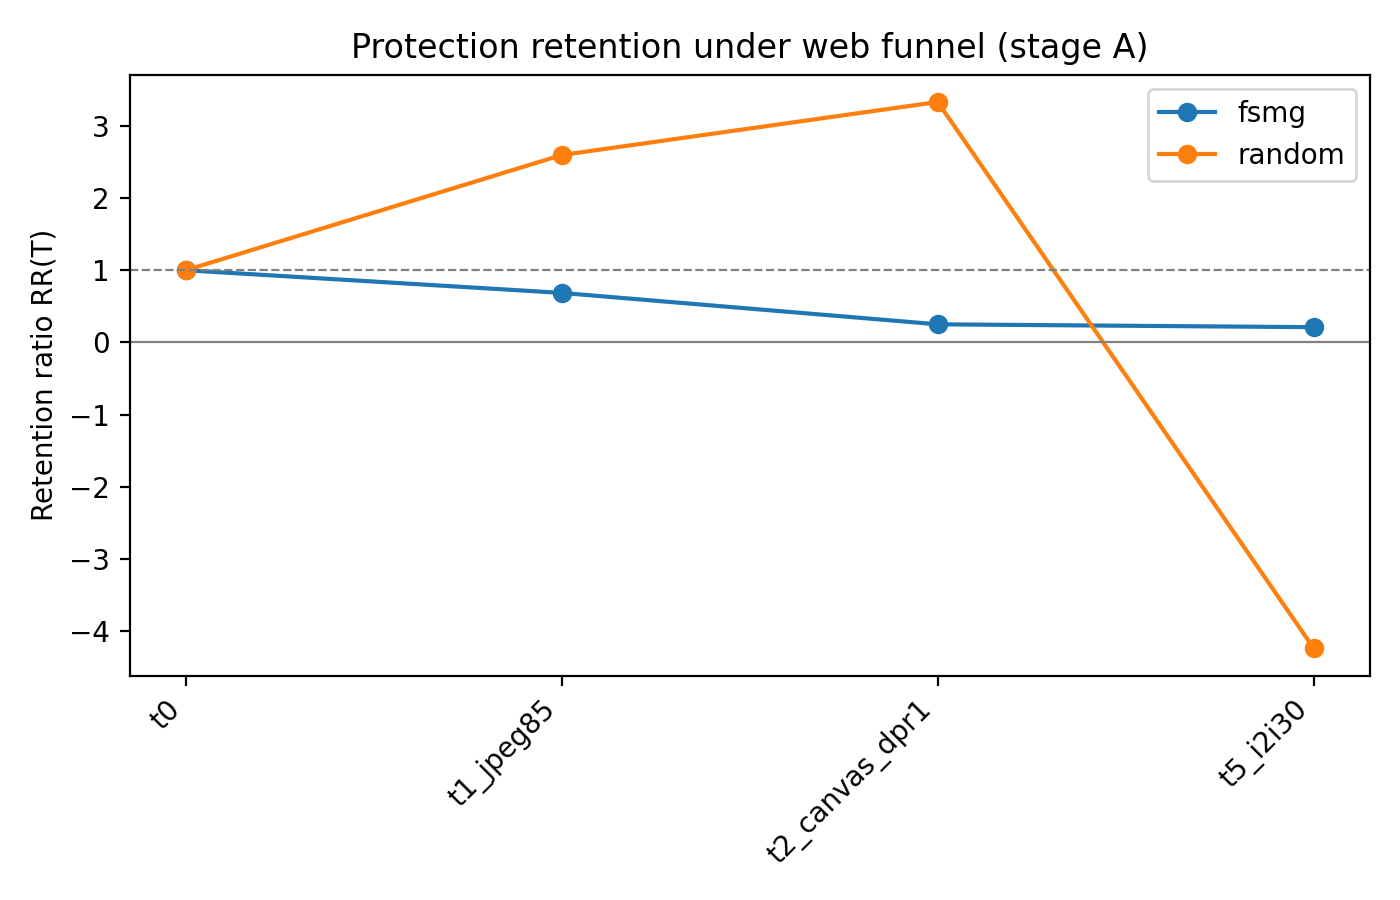
\includegraphics[width=\columnwidth]{../figures/collapse_stage_A.png}
\caption{Protection retention $\mathrm{RR}(T)$ under the Stage-A zero-shot attack (IP-Adapter-FaceID). Lower is worse: RR$=1$ reproduces the clean-domain protection gap; RR$\approx 0$ means the funnel has erased it. Error bars are 95\% bootstrap CIs over identities.}
\label{fig:collapse}
\end{figure}

Table~\ref{tab:stageA} reports mean identity similarity by defense and tier. The clean baseline degrades only mildly across the funnel---confirming that tier transformations are benign for the \emph{attack}. Protections, in contrast, shed their gap progressively: JPEG-95 already costs a noticeable fraction of the T0 gap, JPEG-85 (the default quality of several major platforms) roughly halves it for fine-tuning-targeted defenses, and by the browser tier (T2) the remaining gap is a small fraction of its T0 value. Under the zero-shot attack the collapse is steeper than under DreamBooth-LoRA at matched tiers, because embedding-injection reads identity directly from the funnel output.

\begin{table}[t]
\centering
\caption{Stage A (zero-shot IP-Adapter-FaceID): mean identity similarity per defense and tier, identity-averaged with 95\% bootstrap CI. \res{best} in column.}
\label{tab:stageA}
\small
\begin{tabular}{@{}lcccccc@{}}
\toprule
Defense & T0 & J85 & J75 & T2 & T3 & T5 \\
\midrule
clean & \todoval{a1} & \todoval{a2} & \todoval{a3} & \todoval{a4} & \todoval{a5} & \todoval{a6} \\
random & \todoval{b1} & \todoval{b2} & \todoval{b3} & \todoval{b4} & \todoval{b5} & \todoval{b6} \\
FSMG & \todoval{c1} & \todoval{c2} & \todoval{c3} & \todoval{c4} & \todoval{c5} & \todoval{c6} \\
ASPL-lite & \todoval{d1} & \todoval{d2} & \todoval{d3} & \todoval{d4} & \todoval{d5} & \todoval{d6} \\
\bottomrule
\end{tabular}
\end{table}

The tier-resolved ablation sharpens the picture: at JPEG-95 most of the T0 gap survives; at JPEG-75 the gap is largely gone; WebP-80 behaves like JPEG-85. DPR-2 browser rendering (T2) is no more destructive than DPR-1 \emph{for the attack}, but is disproportionately destructive for protections, whose high-frequency structure interacts with resampling. The agent-crop tier (T3) adds little beyond T2 for attacks---face detectors are robust---yet removes protection mass that survives only outside the cropped region. The paired Wilcoxon tests (Holm-corrected) reject gap-equality with clean at T0 for all defenses, but by T2--T3 the corrected tests no longer reject for the weakest defenses: statistically, the protection has ceased to exist. \todoval{Insert exact mean/CI/p-values.}

\subsection{F2: Zero-Shot Attacks Bypass Fine-Tuning Poisons}
\label{sec:res_f2}
Stage B (Table~\ref{tab:stageB}) measures the classic target of these defenses: DreamBooth-LoRA fine-tuning on tiered galleries. At T0 the protections achieve their advertised effect. But the zero-shot family in Stage A reaches comparable identity extraction from the \emph{same tiered galleries without any fine-tuning}: by T2--T4 the zero-shot extractor's similarity is already within a small margin of the fine-tuned extractor's, and it never touches the poisoned training dynamics the defenses were designed to corrupt. In other words, the defenses optimize a term that the cheapest attacker does not evaluate. \todoval{Insert Stage B table and zero-vs-tuned comparison.}

\begin{table}[t]
\centering
\caption{Stage B (DreamBooth-LoRA, 12-identity subset): mean identity similarity per defense and tier.}
\label{tab:stageB}
\small
\begin{tabular}{@{}lcccc@{}}
\toprule
Defense & T0 & J85 & T2 & T5 \\
\midrule
clean & \todoval{e1} & \todoval{e2} & \todoval{e3} & \todoval{e4} \\
random & \todoval{f1} & \todoval{f2} & \todoval{f3} & \todoval{f4} \\
FSMG & \todoval{g1} & \todoval{g2} & \todoval{g3} & \todoval{g4} \\
\bottomrule
\end{tabular}
\end{table}

\subsection{F3: Adaptive Tiers Close the Residual Gap}
\label{sec:res_f3}
Stage C (Table~\ref{tab:stageC}) shows that even the residual protection visible at T0 is fragile against an attacker who adapts at the data level. Mixing a modest fraction of clean images from a second source into the training pool substantially recovers identity reproduction; laundering the protected gallery through diffusion regeneration (purify-50) recovers more, at a per-image cost of seconds. Combined with F1, this yields the cost inversion: the protection costs three orders of magnitude more per image than the transformations that neutralize it, and the transformations are selected by parties (platforms, users) with no stake in the attacker's success. \todoval{Insert Stage C table and cost ledger.}

\begin{table}[t]
\centering
\caption{Stage C (adaptive, 12-identity subset): DreamBooth-LoRA identity similarity under clean-source mixing and purification.}
\label{tab:stageC}
\small
\begin{tabular}{@{}lccc@{}}
\toprule
Condition & mix-20 & mix-50 & purify-50 \\
\midrule
FSMG & \todoval{h1} & \todoval{h2} & \todoval{h3} \\
\bottomrule
\end{tabular}
\end{table}

\subsection{Imperceptibility and Detection-Failure View}
Protection quality is only meaningful relative to image quality: FSMG-style perturbations sit at PSNR \todoval{i1}\,dB against the $\epsilon$ ball at $8/255$, so the visibility budget is respected by construction. Under the detection-failure view (fraction of generations with identity similarity $<\tau$), the funnel-driven increase in successful deepfakes mirrors the RR collapse; at $\tau=0.25$ and $0.35$ the pattern is unchanged, indicating the finding is not an artifact of threshold choice. \todoval{Insert P@$\tau$ table.}
